\documentclass[11pt,a4paper,fleqn,titlepage,twoside,openany,export]{book}
\usepackage{style}

\subfile{05-slovnik-pojmu}

\bibliography{bibliography}


\begin{document}

\makeatletter
\begin{titlepage}
	\begin{center}
	
	\textsc{\Huge{Univerzita Pardubice}}

	\LARGE{Fakulta elektrotechniky a informatiky}
	
	\vfill
	
	\huge{\@title}\\[2mm]
	\LARGE{\@author}
	
	\vfill

	\begin{normalsize}
	Diplomová práce\\
	2015
	\end{normalsize}
	\end{center}
\end{titlepage}


\newpage  
\thispagestyle{empty}
\begin{center}

\includegraphics[max width=\textwidth,keepaspectratio=true]{imgs-00-zadani/zadani_str_1.png}
\end{center}
\hspace{0pt}

\newpage 
\thispagestyle{empty}
\begin{center}
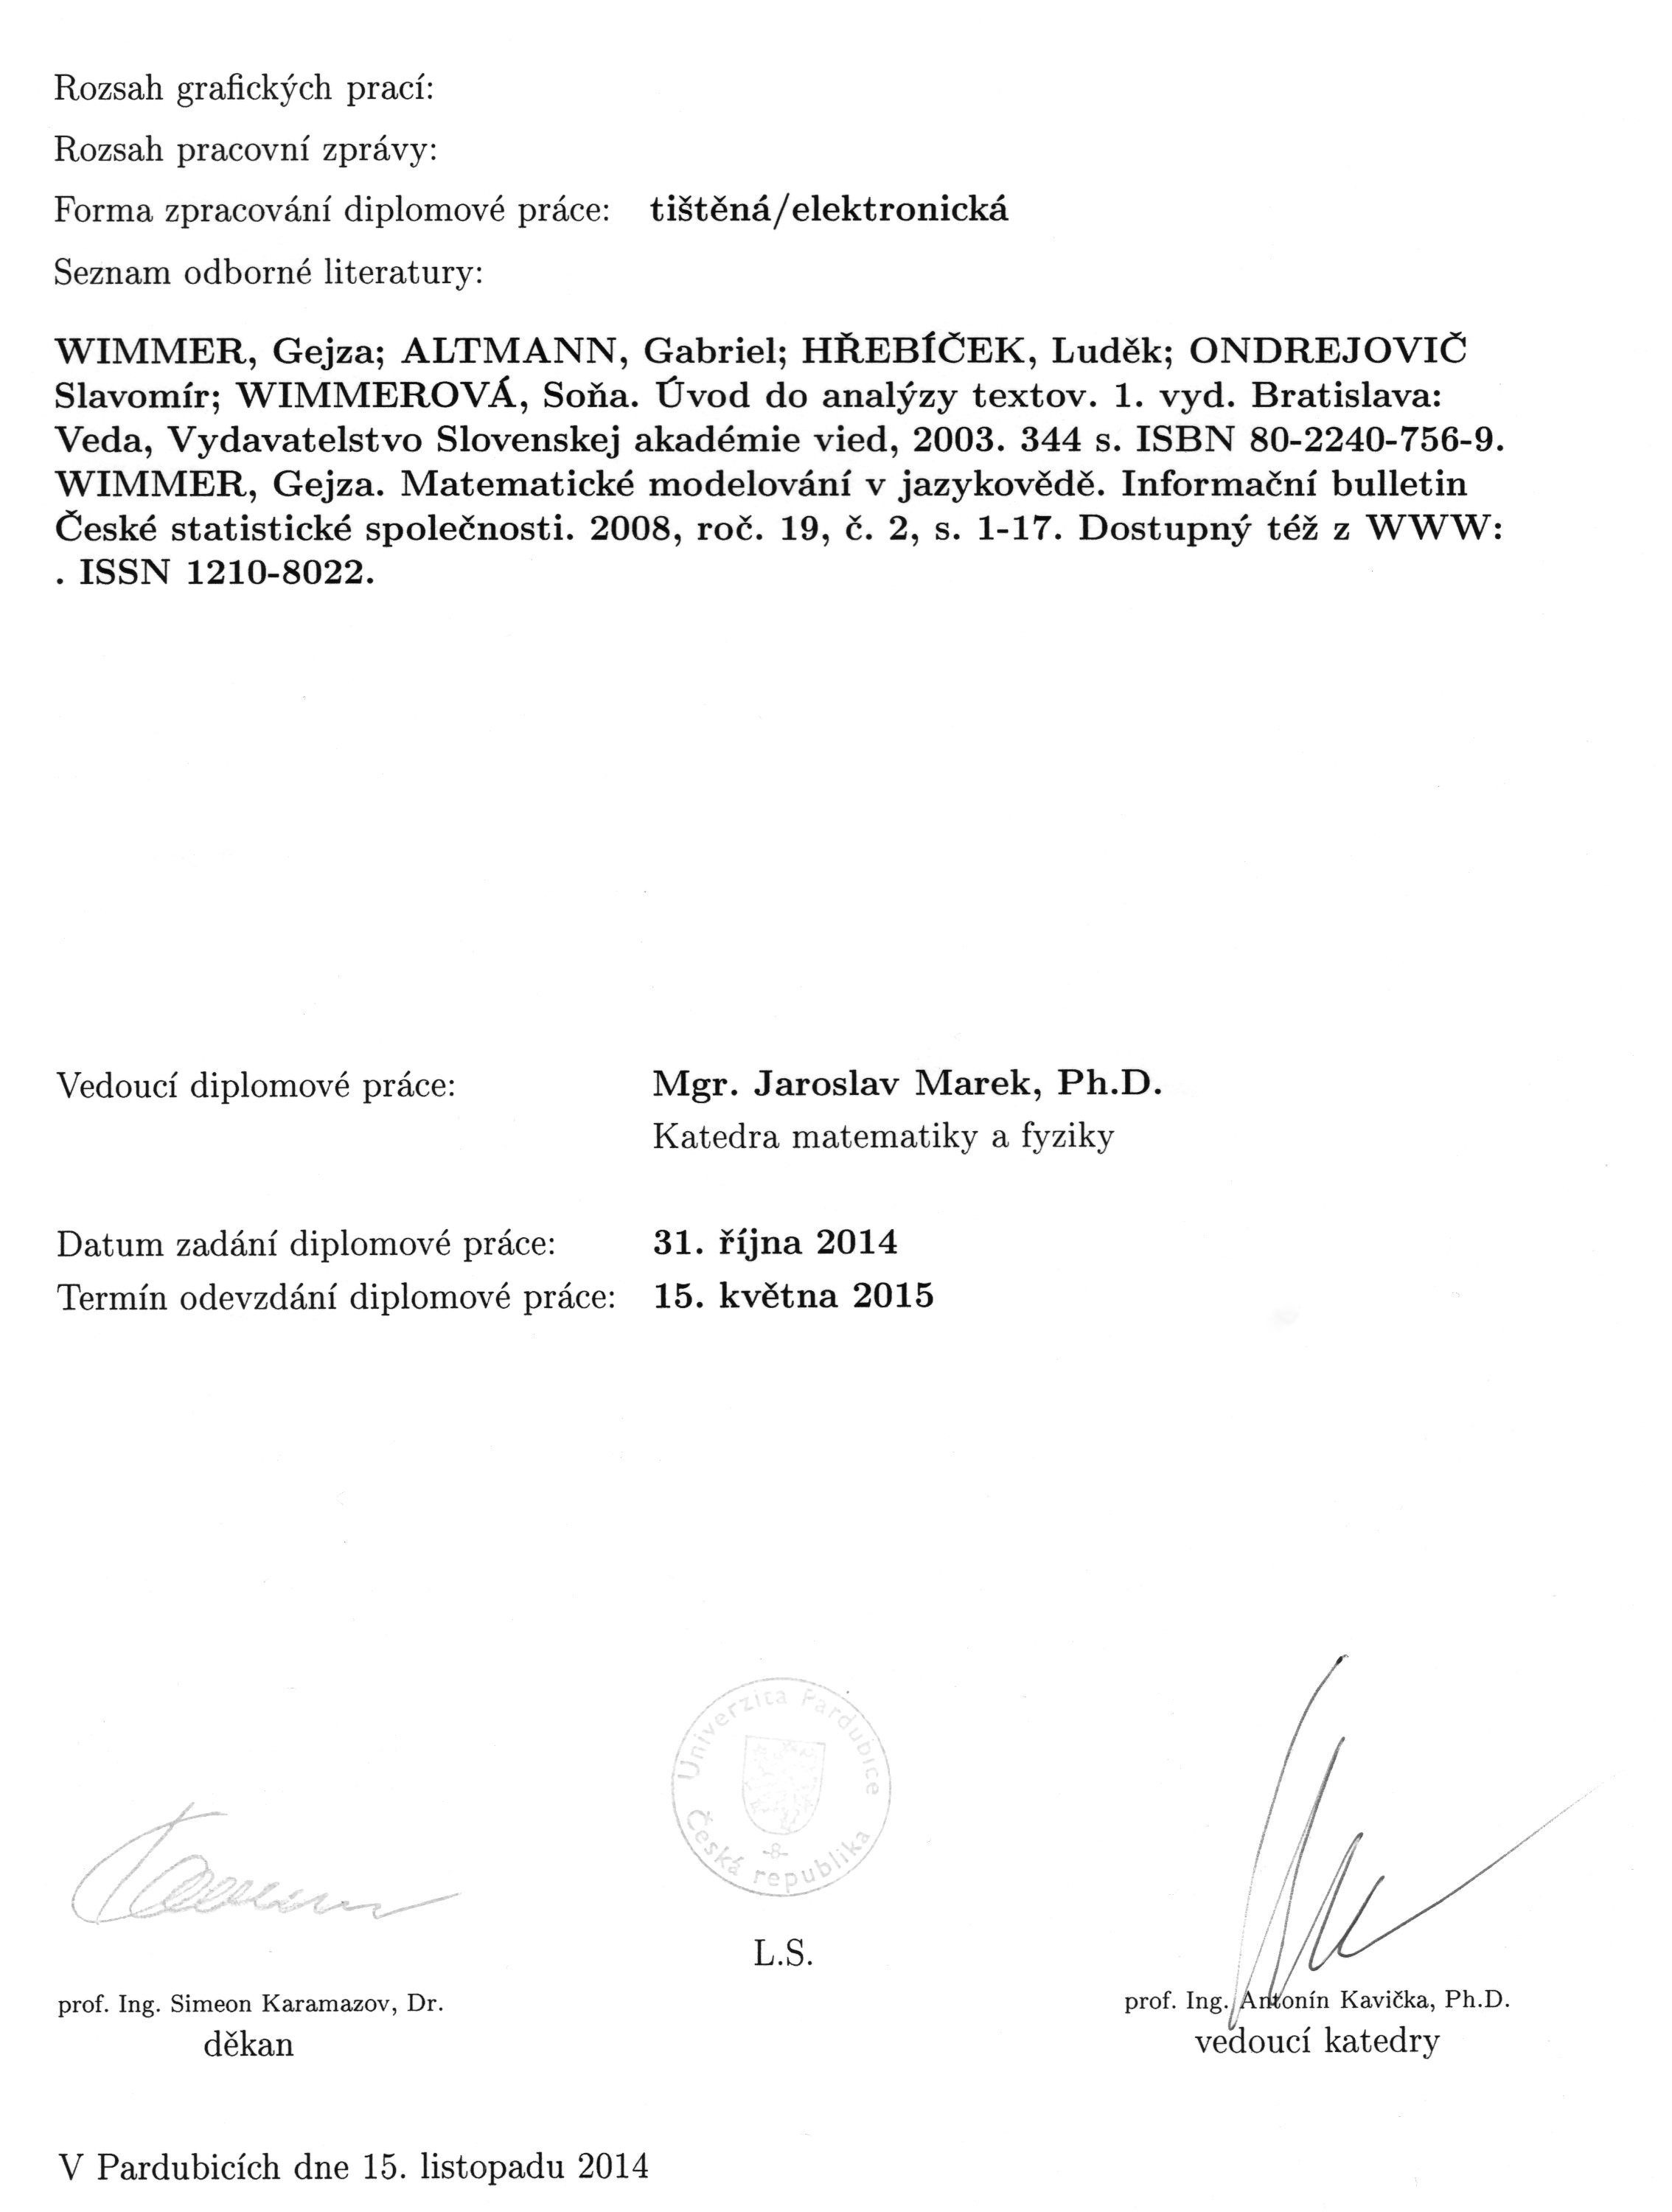
\includegraphics[max width=\textwidth,keepaspectratio=true]{imgs-00-zadani/zadani_str_2.png}
\end{center}
\hspace{0pt}

%\onehalfspacing
\spacing{1.25}

\newpage 
\thispagestyle{empty}
\subsubsection*{Prohlášení autora}

Prohlašuji, že jsem tuto práci vypracoval samostatně. Veškeré literární prameny a informace, které jsem v práci využil, jsou uvedeny v seznamu použité literatury.

Byl jsem seznámen s tím, že se na moji práci vztahují práva a povinnosti vyplývající ze zákona č. 121/2000 Sb., autorský zákon, zejména se skutečností, že Univerzita Pardubice má právo na uzavření licenční smlouvy o užití této práce jako školního díla podle § 60 odst. 1 autorského zákona, a s tím, že pokud dojde k užití této práce mnou nebo bude poskytnuta licence o užití jinému subjektu, je Univerzita Pardubice oprávněna ode mne požadovat přiměřený příspěvek na úhradu nákladů, které na vytvoření díla vynaložila, a to podle okolností až do jejich skutečné výše.

Souhlasím s prezenčním zpřístupněním své práce v Univerzitní knihovně.\\[4cm]
V Pardubicích dne \today\ \hfill{} Jan Šlahora

\newpage 
\thispagestyle{empty}
\subsubsection*{Poděkování}

Děkuji svému vedoucímu panu Mgr. Jaroslavu Markovi, Ph.D. za poskytnuté materiály, čas a cenné rady, bez kterých by tato diplomová práce nikdy nevznikla.

Děkuji i svému tátovi za podporu po celou dobu studia.

\newpage 
\thispagestyle{empty}
\subsubsection*{Anotace}
Práce se zabývá studiem vybraných modelů používaných v rámci matematické lingvistiky a jejich následnou aplikací na české překlady básně Havran amerického autora Edgara Allena Poea. V~rámci práce byl vyvinut počítačový program, který umožňuje aplikovat popisované metody na libovolné texty a porovnávat výsledky sledovaných charakteristik. Součástí práce je i srovnání výsledků jednotlivých metod pro české překlady Havrana.

\vspace*{0.8cm}\subsubsection*{Klíčová slova} 	 	 		

lingvistika, statistika, denotační analýza, fonetické jevy, teorie grafů

\vspace*{2.8cm}\subsubsection*{Title}
Computational linguistics and translations of E. A. Poe's poem The Raven

\vspace*{0.8cm}\subsubsection*{Annotation}

The purpose of this thesis is the study of selected models used within the computational \mbox{linguistics} and their application to the Czech translations of a poem The Raven of an American author Edgar Allan Poe. As a part of the work was developed a computer program which allows you to apply the described methods on any texts and compare the results. The work also includes a comparison of the results of different methods to the Czech translations of the poem The Raven.

\vspace*{0.8cm}\subsubsection*{Keywords}

linguistics, statistics, denotation analysis, phonetic phenomenon, graph theory

\tableofcontents

\let\cleardoublepage\clearpage % vymazání prázdné stránky http://stackoverflow.com/questions/491904/latex-how-to-remove-blank-pages-coming-between-two-chapters-in-appendix

\chapter*{Seznam pojmů a zkratek}
\addcontentsline{toc}{chapter}{Seznam pojmů a zkratek}  

\printglossary[title=Slovník pojmů, nonumberlist]

\printglossary[type=acronym, title=Slovník zkratek, nonumberlist]   

\listoffigures
\addcontentsline{toc}{chapter}{\listfigurename} 

\listoftables
\addcontentsline{toc}{chapter}{\listtablename} 

\thispagestyle{empty}

\subfile{00-predmluva}
\subfile{10-uvod}
\subfile{50-denotacni-analyza}
\subfile{60-aplikace}
\subfile{70-experiment}
\subfile{99-zaver}


\printbibliography[title={Seznam použité literatury},heading=bibintoc]

\appendix
\subfile{99-appendix}


\end{document}